\documentclass[a4paper,10pt]{article}
\usepackage[T2A]{fontenc}
\usepackage[utf8x]{inputenc}
\usepackage{ucs}
\usepackage{cmap}
\usepackage[english,russian]{babel}
\usepackage{amsmath}
\usepackage{color,graphicx}
\usepackage{indentfirst}

\title{SRM методичка}
\author{Чернышев Алексей}
\setlength{\parindent}{1cm}

\begin{document}
\section*{Спайковые НС}
\section*{Spike Responce Model}
\paragraph*{Общее описание. }Spike Responce Model (SRM) - наиболее популярная модель спайкового нейрона. SRM своей популярностью обязана простотой математической интерпретации - вся динамика нейрона описывается одним уравнением вида $u(t)$, которое описывает напряжение на мембране нейрона и, по сути, является решением дифференциального уравнения для моделей типа \textit{Integrate and fire}. Динамику моделей \textit{Integrate and fire} можно описать так: нейрон суммирует входные сигналы и по достижению определенного порога, производит спайк, после чего нейрон переходит в состояние рефракторности, находясь в котором, вероятность нового спайка крайне мала.\\
\indent Поведение описанное выше можно поэтапно собрать в одну формулу: 
\begin{enumerate}
\item \textit{Функция описывающая напряжение на синапсах}. В качестве такой функции можно взять альфа функцию с экспоненциальным подъёмом и спадом, причем подъем и спад наиболее натуральным будет взять быстрым и медленным соответственно. Типичный график подобной функции можно посмотреть на рисунке ниже:
\begin{figure}[ht]
\centering
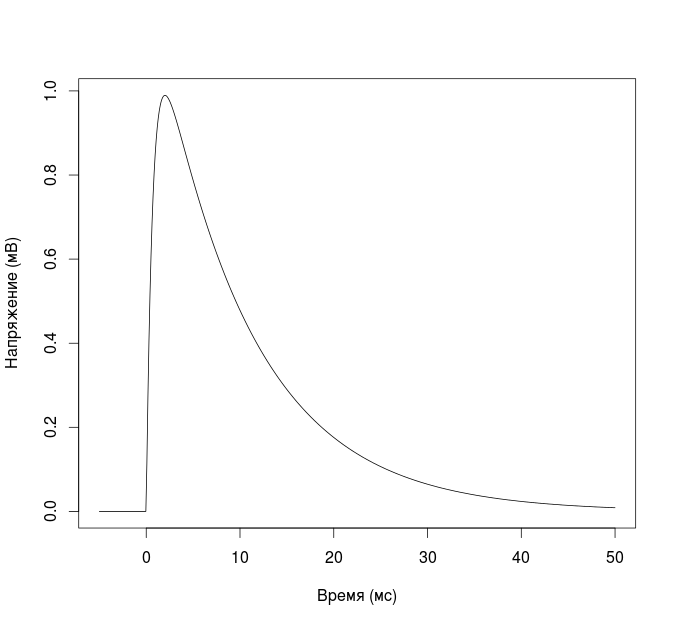
\includegraphics[width=0.75\linewidth]{epsp}
\caption{Потенциал на синапсах}
\end{figure} \\
Такая функция задается формулой:
\begin{equation}\label{eq:epsp}
\epsilon(t) =	\epsilon{0}(\exp(-t/t_{m})-\exp(-t/t_{s})),
\end{equation}
где $\epsilon{0} = 1.3$мВ - контанста задающая масштаб потенциала, $t_{m}=0.7$мс - константа отвечающая подъем, $t_{s} = 10$мс - константа отвечающая спад.

\item \textit{Функция описывающая рефракторность нейрона}. Основное требования к такой функции в том, чтобы напряжение на нейроне резко падало вниз, и потом медленно восстанавливалось. График подобной функции можно увидеть на рисунке ниже:
\begin{figure}[ht]
\centering
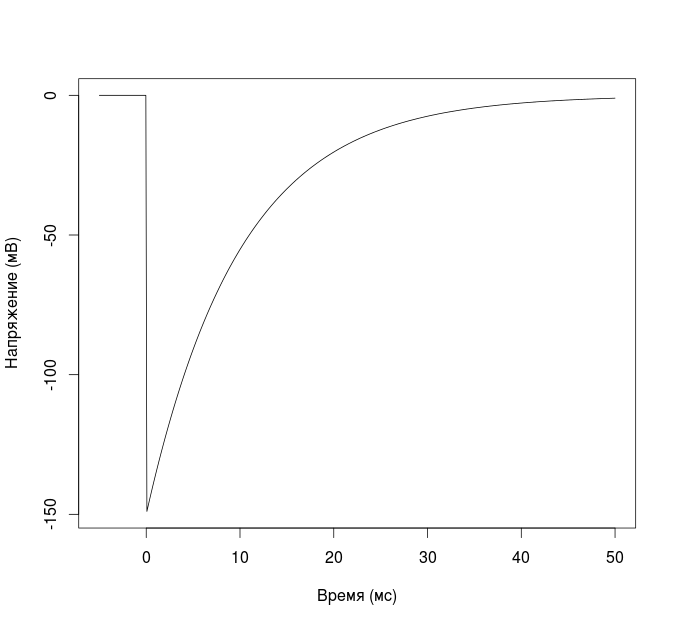
\includegraphics[width=0.75\linewidth]{nu}
\caption{Рефракторность нейрона}
\end{figure} \\
Здесь используется данная функция:
\begin{equation}\label{eq:nu}
\eta(t) =	\eta_{0}(-\exp(-t/t_{m})),
\end{equation}
где $\eta_{0} = -150$мВ - констанста описывающая минимальное напряжение на мембране, от которого идёт медленное восстановление, $t_{m}$ - скорость восстановления можно взять из функции синаптического потенциала, для простоты. 
\end{enumerate}
В итоге, используя эти функции, можно записать уравнение, которое будет описывать напряжение на мембране нейрона, причём: \\
\begin{itemize}
 \item Пусть нейрон $i$ имеет $N$ синапсов и у каждого синапса есть вес $w_{i}$, тогда напряжение на мембране в данный момент времени $t$ будет взвешенной суммой синаптических потенциалов: $\sum_{j=1}^N w_{j} \sum_{f_{j}} \epsilon_{j}(t-f_{j})$, где $f_{j}$ - время спайка на синапсе $j$. \\
\item Рефракторность нейрона будет простой суммой по всем спайкам, которые произвел нейрон $i$: $\sum_{f_{i}}\eta(t-f_{i})$
\item Нейрон имеет т.н. потенциал покоя. Биологические нейроны имеют разнообразные значения такого потенциала, как правило берут $u_{rest} = 70$ мВ.
\end{itemize}

\indent Таким образом получаем формулу, которая объединяет все вышеописанные особенности:
\begin{equation}\label{eq:u_srm}
u(t) = u_{rest} + \sum_{j=1}^N w_{j} \sum_{f_{j}} \epsilon_{j}(t-f_{j}) + \sum_{f_{i}}\eta(t-f_{i}),
\end{equation}
Типичный график иллюстрирующий работу функции \ref{eq:u_srm} ниже: 
\begin{figure}[ht]\label{pic:u_srm}
\centering
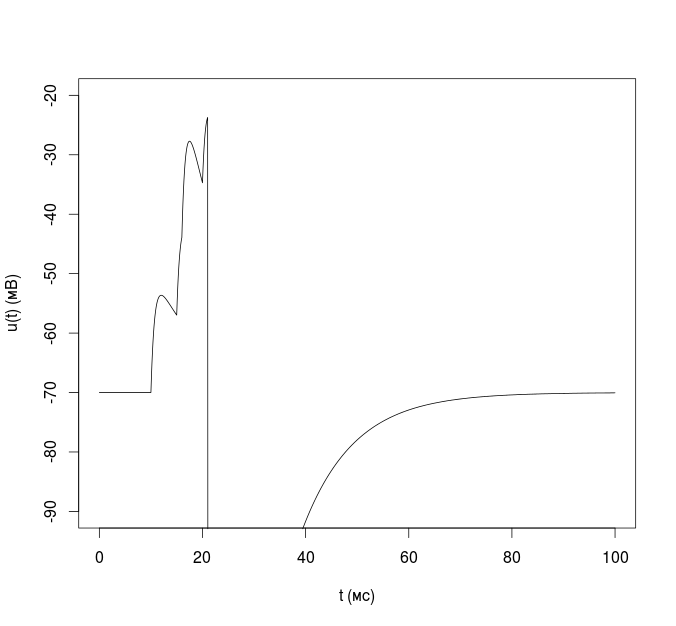
\includegraphics[width=1\linewidth]{u_srm}
\caption{Потенциал нейрона}
\end{figure} \\
\indent На рисунке представлен случай когда произошли спайки на двух синапсах во времена $f_{1} = \{10, 16\}$ и $f_{2}=\{15,20\}$, которые заставили нейрон произвести спайк в $f_{i} = \{21\}$. Веса были выбраны большими, для наглядности графика.
\paragraph*{Генерация спайков.} Модель описанная выше включает в себя только поведение при данных временах спайков на синапсах нейрона и самого нейрона. Рассмотрим вопрос условия генерации спайков.\\
\indent Классическим вариантом модели генерации спайков является модель с порогом напряжения. Т.е. при достижении нейроном какого-то конкретного порогового напряжения - нейрон генерирует спайк. Как показала практика, наиболее удобным в математическом анализе таких моделей является стохастическая модель порога. Особенность такой модели в том, что нейрон генерирует спайк с определенной вероятностью, которая всё же зависит от напряжения на мембране и которая делает резкий скачок около порогового напряжения. Пример такой зависимости на рисунке ниже:
\begin{figure}[ht]\label{pic:p_srm}
\centering
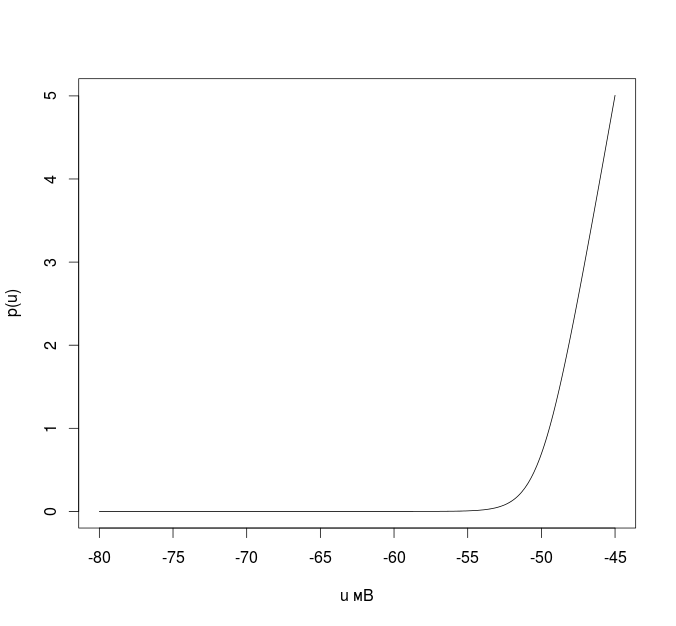
\includegraphics[width=1\linewidth]{p_srm}
\caption{Плотность вероятности генерации спайка}
\end{figure} \\
\indent Такая плотность вероятности является ненормализованной, т.к. её интеграл больше единицы, и имеет все свойства плотности вероятности Пуассоновского процесса. Например, вероятность генерации одного спайка в отрезок времени $\Delta t$ будет $P = p(u(t))\Delta t$.
\paragraph*{Математический фреймворк.} Используя выкладки выше можно вывести математическую базу для Spike Responce Model. Ниже приведены основные формулы.
\begin{itemize}
\item \textbf{Вероятность отсутствия спайков в диапазон $[0,T]$ при данных спайках на синапсах $X$ ($Y_{0} = \{\} $)}:
\begin{equation}\label{eq:p_y}
P(Y_{0}|X) = S[0,T] = \int_{0}^{T} exp(-p(t))dt\;,
\end{equation}
\\
\item \textbf{Вероятность генерации спайка в момент времени $t_{f}$ диапазоне $[0,T]$ при данных спайках на синапcах $X$.}
\begin{equation}\label{eq:p_y}
P(Y|X)= S[0,t_{f}]\; p(t_{f})\; S[t_{f},T]\;,
\end{equation}
\item \textbf{Вероятность генерации спайковой последовательности $Y = \{t_{f1},t_{f2},..,t_{fn}\}$ диапазоне $[0,T]$ при данных спайках на синапcах $X$.}
\begin{equation}\label{eq:p_y}
P(Y|X)= S[0,t_{f1}]\; p(t_{f1})\; ...\;S[t_{fn-1},t_{fn}]\;p(t_{fn}) \; S[t_{fn},T],
\end{equation}
\end{itemize}
\end{document}
